\chapter{Introduction and Background}\footnotetext{some content in section 1.1 and  section 1.2 of  this  chapter is adapted from Dou, Yong, Kiran Dhatt-Gauthier, and Kyle JM Bishop. "Thermodynamic costs of dynamic function in active soft matter." Current Opinion in Solid State and Materials Science 23.1 (2019): 28-40.See appendix for the full text of this paper}
Robotics is in the spotlight of coming industry 4.0 era \cite{lasi2014industry}.Highly automatic robots will largely increase the productivity and efficiency in many areas such as manufacturing, transportation and retailing. 
It is predicted that 47$\%$ percent of jobs will be replaced by robotics in two decades. \cite{frey2013future}
Research on robotics almost include all part of science and engineering fields from the data science, machine learning to the material science and biology. Lots of current design and development of robotics are inspired from nature to achieve the animal/human-like functions, for example  the famous  bio-inspired robot SPOT\textregistered  by Boston Dynamics \cite{yang2019ten} can perform like dogs  to climbs stairs and run on rough terrain with very impressive ease. Normal robots are usually in the size of meters. However, this dissertation is going to focus on robots with a much smaller size around microns(1$\mu m=10^{-6} m$) called \textbf{colloid robots}. Colloid robots are at the same size of microorganism and living cells,and are designed to mimic similar living functions in a colloidal scale.  

In the first chapter, some basic knowledge of colloid robots are introduced as well as the state of arts research on colloid robots. We gave the  classification for colloid robots based on different automation level(from level 0 to level 6). Chapter 2 showed  an example example developed by us to a achieve level 1 automation with electrostatic actuation. Contact charge electrophoresis(CCEP) uses the repeating electrostatic charging and actuation to drive   
continuous autonomous motion of anisotropic colloids particles with very high speed and low power input. In Chapter 3, we  design an experiment system that conductive  colloids particles can interact with each other to generate dynamic travelling waves. A modified Kuramoto model treating colloids as phase oscillators is proposed to explain the experiment observation. Chapter 3 provide a pathway to realize level 2 automation for colloid robots. In Chapter 4, a theoretical toy model is introduced to design level 4 automation colloid robots. The colloid robots are interact with the environment and make decisions based on local information by changing their shapes to reach the global navigation behaviors. This toy model provides an design and optimization frames for autonomous navigation in colloid robots. Chapter 5  shows a system in which  magnetic actuated colloid robots can  finish level 4 autonomous navigation. We develop physical mode of     magnetic actuated colloid robots and optimize the design space to navigate the motion of magnetic rollers.  Preliminary experimental results are also discussed in chapter 5. In Chapter 6, future research directions  are proposed  to guide  ultimate realization of  automation level 5 and 6 colloidal robots. 

\section{Bio-inspired Colloids Robots}
Living cells or microorganism(e.g. bacteria) are the smallest unit of life. Although these smallest units is only in the size of colloid particles(most cells' size are in the range from 1$\mu m$ to 100$\mu m$), living cells can perform all the basic remarkable dynamics functions of life. For example, plan cells capture energy from sunlight and convert it into chemical fuels and structural materials; muscle cells powers organisms to move and to transport matter throughout their interiors; the cytoskeleton incessantly reconfigures its structural components, enabling cells to adapt their mechanical properties to their environment; neural cells uses complex signaling networks to sense environmental inputs and compute intelligent outputs. Perhaps most remarkably, all cells can grow and replicate to escape the unrelenting pull toward thermodynamic equilibrium (i.e., death).  All of these functions ---and the many others not listed---would be highly desirable to achieve in an small artificial robotics system, or called as colloids robots. \textbf{Colloids robots refers to the colloid size units which can perform life-like autonomous behaviors including motion, navigation, sensing, communication or even high level cognition}.  Colloids robots are bio-inspired and trying to mimic living cells, however colloids robots can also designed to have better performance and more complex functions than real living cells. A qualified colloids robots is designed to finish colloid scale tasks with high accuracy and precision at a reasonable energy efficiency.

\begin{figure}
\centering
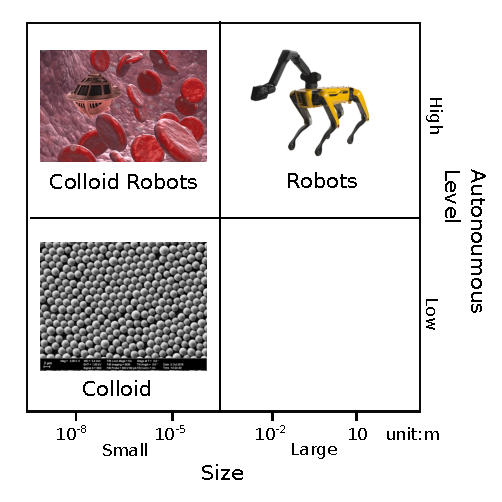
\includegraphics[width=9cm]{figures/1_1.pdf}
\caption{Colloid robots}
\label{fig:1}
\end{figure}

\section{Why colloids Robots are different and could be hard to realize}
Although colloids robots still follow the basic control feedback of normal size robots: sensing, computation and actuation, these components of the control loop are hard to realize with respect to the size limitation and totally different physics in small scale. 

\textbf{Size limitation}. In addition to the three basic components( sensor,actuator and processor) in the feedback loop, a robot also need power supplies, manipulators with joints and a body frame etc. Even for a simple clean robots, there are around 100 parts inside. It is not possible to integrate all of these complex components in a micron size(a micron size particle on a cleaning robot is just like a human standing on the earth) particle if we follow the common way to build a normal size robot. 

\textbf{Physics limitation}. Physics in a small scale and squishy  environment is very different from our normal size world, where everything becomes noisy and sticky. First, in the colloidal scale, Brownian motions largely affect the dynamics of colloidal particles, adding stochastic influence to the robotics. These thermal motions increase the difficulties in controlling colloid robot's accuracy and precision. Second the inertia totally disappear in the small scale as the Reynolds number of the colloid robot's system approach 0.  Reynolds number presents the ration of inertia and viscosity represented as
\begin{equation}
    Re=\frac{\rho v l}{\mu}
\end{equation}
where $\rho $ is the density of fluid environment, v is the velocity of particle, l is the size of particle. $\mu$ is the  viscosity of fluid. In the colloid scale, both size and speed of particle are much smaller than 1 leading to the Reynolds number approach 0. The absence of inertia means all of the actuation method in normal size robots based on inertia will no longer work. This interesting  motion restriction in low Reynolds number is called Scallop
theory and was first discussed by Edward Purcel(Professor Prucel was famous for his independent discovery of something else(nuclear magnetic resonance,NMR), which brought him a Nobel prize) \cite{purcell1977life}. As shown in \textcolor{red}{fig XXX},  Scallop Theorem states that a swimmer that exhibits time-symmetric motion cannot achieve net displacement in a low Reynolds number fluid environment because all the motion is time reversal like the open and close of a scallop. New actuation methods must be applied to drive motions for colloid robots.

To solve the above mentioned problems and design colloid robots, researchers got inspired from living. The dynamic functions of living cells require integration of structures and processes to drive material organization in space and time. For example in muscle cell,  the coupling of complex structures(kinesin motor protein) and dissipative processes (ATP hydrolysis) can generates mechanical work. \textcolor{red}{see fig XXX}

Thanks to the development of nano/micro scale fabrication in semiconductor industry, we can now create materials with heterogeneous structure and composition on length scales spanning molecular to macroscopic dimensions with chemical synthesis, lithography, deposition and etching. These technologies can be directly transplanted to the fabrication process of colloidal robots. In addition to structural and material complexity, the artificial dissipation process(or actuation process) for colloid robots  can be generated  with chemical reaction, external field(electric, magnetic, acoustic or fluid flow) to generate motion by by break the time reversal physics. For past decade, lots of research has been conducted to design colloidal robots or study the fundamentals of colloid robots. Colloid robots is now a very hot emerging interdisciplinary field attracting many scientist from math, physics, chemistry, biology and engineering. The states of art of  research approach to colloid is reviewed on\textcolor{red}{section , section }
\section{Difference between a colloid machine and a colloid robots}
 Some research proposed the idea of colloid machine which can also harness energy from environment to perform dynamics motions such as motions and assembly.\cite{spellings2015shape,van2016spatiotemporal} 
 So before we introduce more about colloid robots, we would like make clear explanation for the definition of  colloid robots and why colloid robot is unique. Generally,although showing some level of autonomous, a machines is only a part or an very early stage  of a fully intelligent robot.\cite{whitesides2018soft} We can borrow the standard in industry robot's ISO definition.\cite{virk2008iso}
A colloid robot must be capable of \textbf{programmable} for \textbf{multipurpose} task and controlled automatically in a colloid scale.  The key difference between machine and robots are re-programmable and re-purposable:
\begin{itemize}
    \item Re-programmable: Colloid robots' motion and interactions could be changed without core physical or chemical renovation via sensing feedback loop.
    \item Re-purposable: Colloid robots' could be used in various environment for different tasks  such as different directions' navigation via re-programming.
    \item Physical  and chemical renovation:  rebuilt the colloid robots with different principles such as different chemical reactions or different physical interaction.
\end{itemize}
If you can't easily re-purpose colloid machine to do something completely different by reprogramming (making minimal hardware "tool" changes) easily as well, the colloid machine is not a really colloid robots.
For example, a hammer is a machine that you can put it in the assembly line to drive a small nails.   Or we could add a computer vision system to hammer coupled with hammers' actuator. Now the hammer is a robotics hammer. The hammer can adapt the drive force based on different size of nails--smaller nail with small force, larger hammer with large force. As a robotics hammer, it can also be reprogrammed without much efforts to the opposite rule--smaller nail with large force, larger hammer with small force. When not used to drive nails, this hammer can also be applied to other jobs such as breaking parts.


\section{Automation level of Colloid Robots}
Before the review of current approach to the colloid robots, 
we give the  automation level definitions for colloids robots,  analogy to the Levels of driving automation\cite{taeihagh2019governing}. This level definition is proposed to guide the research road-map for colloid robots.
\begin{itemize}
    \item Level 0 No Automaton: This level of automation means colloid robots cannot do anything autonomous. All the conventional colloid particles (even with complex structures and components) belong to this level. These particles are in the equilibrium state.
    \item Level 1 Autonomous  Motion: At level 1, individual colloid robot can continuous harness the energy from the environment to power autonomous motion. This is the entry autonomous level for colloid robots. Although colloid robots at level 1 can move, they can't move with any complex tasks such as navigation and communication.
    \item Level 2 Autonomous Coordination: Group of colloid robots can interact with each other to perform swarm behaviors and generate patterns. Colloid robots begin to show the sensing function at Level 2 via interacting with each other. But this kind is sensing is passive  and still lack the ability to make initiative decision/reaction based on sensing. 
    \item Level 3$^{-}$ Supervised Autonomous Navigation (Eyes on): colloid robots' motion can be guided with the outside computer vision feedback system. At Level 3$^{minus}$, the sensor are outside the colloid robot as the observation microscope, camera. The decision makers and respond mechanism are supervised by outside computer vision algorithm. Colloid robots cannot finish navigation task independently in a small scale.
    \item Level 3$^{+}$ Unsupervised Autonomous Navigation (Eyes off): Colloid robots can finish the sensing-computation-actuation feedback loop independently without the outside devices to supervise. Autonomous navigation in Level 3 $^{+}$ satisfied the basic autonomous requirement for a normal robot. Autonomous level higher than level 3 will enter the area of artificial intelligent.
    \item Level 4 Autonomous Communication: At the level 4 automation, colloid robot can not only sense the information from their local environment, but can also communicate with other colloid robots, sharing&transporting information to make decision together. Autonomous communication will significantly increase the efficiency of colloid robots' job such as searching and repairing.
    \item Level 5 Colloid Artificial Intelligent: This level colloid robots need \textbf{0 human input} to finish any desirable tasks after created. Level 5 colloid particles are also likely to show some high level-like functions such as 
    growing, learning, cognitive abilities  even reproduce.
\end{itemize}
One thing need to mention here is that the technologies development stages are not linear but exponential instead. Higher level automation of colloid robots  represent much more research efforts and could take longer to reach higher autonomous level states.

\begin{table}[h!]
  \centering
  \begin{tabular}{ | m{6cm} | m{6cm} | }
    \hline
    Automation Level & Illustration \\ \hline
    %\begin{minipage}[t]{5cm}
     0.No Automaton
    %\end{minipage}
      &
      \begin{minipage}{.3\textwidth}
      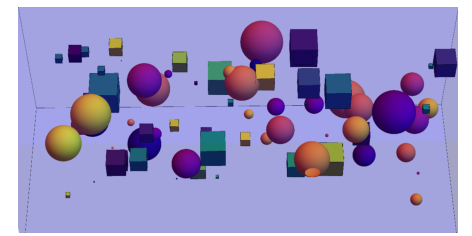
\includegraphics[width=\linewidth]{figures/table1_1.pdf}
    \end{minipage}
    %\end{minipage}
    \\  \hline
    %\begin{minipage}[t]{5cm}
      1. Autonomous Motion
    %\end{minipage}
  
      &
      \begin{minipage}{.3\textwidth}
      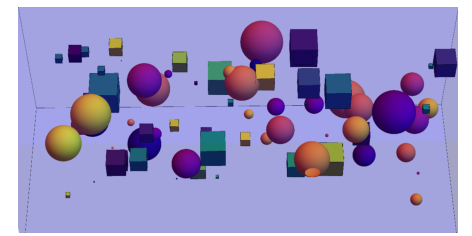
\includegraphics[width=\linewidth]{figures/table1_1.pdf}
    \end{minipage}
    %\end{minipage}
    \\  \hline
    %\begin{minipage}[t]{5cm}
      2.Autonomous Coordination
    
      &
      \begin{minipage}{.3\textwidth}
      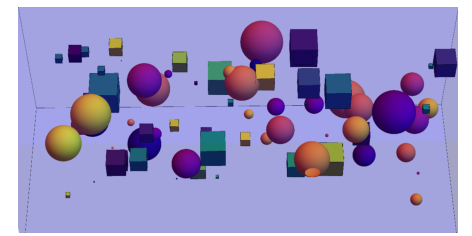
\includegraphics[width=\linewidth]{figures/table1_1.pdf}
    \end{minipage}
    %\end{minipage}
    \\  \hline
    %\begin{minipage}[t]{5cm}
      3$^{minus}$. Supervised  Autonomous  Navigation  
    
      &
      \begin{minipage}{.3\textwidth}
      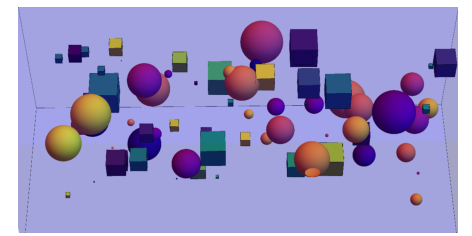
\includegraphics[width=\linewidth]{figures/table1_1.pdf}
    \end{minipage}
    %\end{minipage}
    \\  \hline
    %\begin{minipage}[t]{5cm}
      3$^{plus}$. Unsupervised Autonomous Navigation 
   
      
      &
      \begin{minipage}{.3\textwidth}
      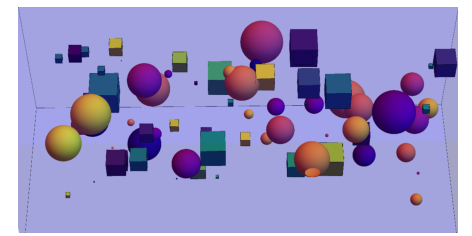
\includegraphics[width=\linewidth]{figures/table1_1.pdf}
    \end{minipage}
    %\end{minipage}
    \\ \hline
    %\begin{minipage}[t]{5cm}
      4. Autonomous Communication
    
      &
      \begin{minipage}{.3\textwidth}
      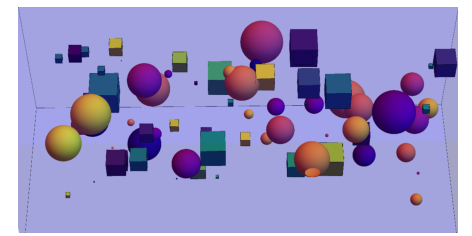
\includegraphics[width=\linewidth]{figures/table1_1.pdf}
    \end{minipage}
    %\end{minipage}
    \\ \hline
    %\begin{minipage}[t]{5cm}
      5. Colloid Artificial Intelligent: 
  
      &
      \begin{minipage}{.3\textwidth}
      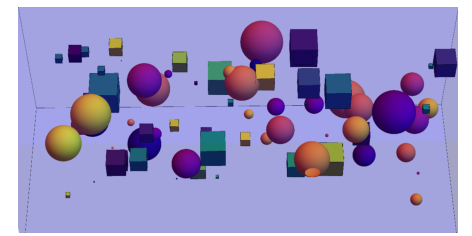
\includegraphics[width=\linewidth]{figures/table1_1.pdf}
    \end{minipage}
    %\end{minipage}
    \\ \hline
    
    
    
  \end{tabular}
  \caption{Automation level of colloid robot}\label{tbl:myLboro}
\end{table}



\section{A state of art review on colloid robots }
It is not clear which paper first mentioned  similar idea of colloid scale robotics(the basic concept of  small scale machines can be tracked to Richard Feynman's famous paper,\textit{There's plenty of room at the bottom}\cite{feynman1960there}). The current research wave in the past decade on colloid robot is triggered by the discovery of self propulsion active colloid particle in chemical fuels \cite{paxton2004catalytic}. In 2004, scientist from Penn State University found chemical fuel(they use hydrogen peroxide, $H_2O_2$ in the first paper) can drive  gold-platinum bimetallic nanorods' autonomous motion. The asymmetric different chemical reactions , which happen at different end of nanorod,  lead to a net flow fluid near the surface of nanorod. This pioneer research then attracted lots of attention in different research field beyond chemistry such as soft condensed matter physics\cite{Marchetti2013}, materials science\cite{han2018engineering}, applied math\cite{fodor2016far} and engineering research\cite{sitti2015biomedical}. More than tens of thousands papers related to the autonomous behaviors of colloids have been published since then. However, most of these research papers either experiment or theory only realize the first 2 level automation(autonomous motion and coordination) in colloid robots. Only a few of them realize the supervise/unsupervised autonomous navigation function. From our knowledge, the higher level's automation is still challenging, and should be the main research direction in the future. In the following content, we are going to give a short state-of-art of art review on both experiment approach to colloid robots as well as new theories and simulation methods towards colloid robots. In this short review, I have no intention and interests to rephrase and cover all the research papers on colloid robots like an encyclopedia book. Instead,  I will focus on the main physics, chemistry and engineering ideas behind these papers. The current experiment approach and theory are also summarized in \textcolor{red}{figure and figure}  

\subsection{Experiment Approach}

\textbf{Fabrication}  High throughput nano/micro scale fabrication technologies in semiconductor manufacturing industry now can make 3-D structure even smaller than 5$nm$.\cite{mokhlesi2010three} These fancy technologies to make CPU and memory can be transplanted directly to make colloid robots of almost any desired size, shape and component in clean room.\cite{koman2018colloidal} A typical fabrication process mainly including lithography to make patterns as sacrificing models, etching to remove unnecessary materials and deposition to introduce new materials. Multi-layer processing can be designed and optimized to make high dimension and complex structure such as spiral shape\cite{zhang2009artificial}. After the colloid robots are fabricated on the wafer, they can be harvested from the silica surface with etching technology or simply physical removal. For the detailed process of fabrication, I would like to refer readers to these 3 comprehensive reviews\cite{wong2016synthetic,wang2017emerging, zha2018tubular}. Chemists and material scientists also contributed creative chemical synthesis methods to make colloid scale complex structure with one-pot high-throughput\cite{youssef2016shape,gong2017patchy,wang2019active}. One challenge for colloid robot's fabrication is to   make  colloid scale soft(or shape changing) structure with complex component component. liquid crystal, hydrogel gel, droplet and silica polymer with self assembly property are promising candidate materials for micro/nano scale soft structure. \cite{leong2009tetherless,denkov2015self,zhang2017printing,wei2019molecular}. Another fabrication challenge is to make bio-hybrid colloid robots,where experimental biologist can provide invaluable experience and knowledge.\cite{stanton2016biohybrid,magdanz2013development}

\textbf{Actuation} Autonomous motion is the most fundamental characteristic of colloid robots, making colloid robots real machines instead of simple colloid particles. Colloid robots can harness energy from environment and convert energy into mechanical work. Compared to the inertia driven mechanism in normal size robot, the actuation of colloid robots always experiencing large hydrodynamics resistance force to balance the driving force. The actuation's power source can be divided into two main category: chemical/biochemical reactions and the external physical fields. Living cells and bacteria use a series of  chemical reaction networks (e.g. ATP hydrolysis) to convert their food source to motions. Colloid robots can also mimic this life-like energy conversion mechanism by designing and tuning the reactions on the surface with their fluid environment. Colloid robots can work as catalyst or reactant to trigger the reaction in fluid environment. For example,  colloid robots can be made of gold or metal  which catalysis the hydrogen peroxide in the fluid to water and oxygen. During the fabrication process, these catalysis or reactant material are patterned at different place of colloid robots to break the symmetry in low Reynolds number environment with chemical species' gradient or reaction product(e.g. bubbles) \cite{velegol2016origins,shklyaev2016harnessing,parmar2018micro}. Recent reports also showed biochemical reaction(e.g. enzyme) can be options to drive colloid robot's motions.\cite{zhao2018substrate,somasundar2019positive}.

In addition to  chemical reactions, almost all the external physical field have been used to powering autonomous motion of colloid robots including electric\cite{lee2019directed}, magnetic\cite{zhang2009artificial}, acoustic\cite{sabrina2018shape}, light\cite{dai2016programmable}, or thermal field\cite{lozano2016phototaxis}.  Colloid robots programmed with physical monopole, dipole or quadrupole will response to the external physical fields, leading to rotational or transitional motion. For example, colloid robots can be fabricated with magnetic materials such as nickel and cobalt to have magnetic dipole. Then an external magnetic can accurately manipulate the motion of magnetic colloid robots.Compared to the  chemical reaction method, external physical field can drive colloid robots with less fluctuation trajectories  \cite{han2018engineering,ren2018two}. 
The current defect in actuation of colloid robots is the very low energy efficiency(usually in the order magnitude of $<10^{-5}$ or less). Colloid robots always dissipate large amount of heat\cite{wang2013understanding} compared to the real living cells that can perform efficient motion with much less heat dissipation.

\textbf{Coordination}  Colloid robots have shown some extent of coordination via interaction and coupling. They can perform some life-like collective behaviors such as  birds' swarm and fish's flock \cite{wang2015one,ginot2018aggregation}. Emergent patterns ,dynamic clustering and phase separation have been observed  in different colloid robots systems. \cite{buttinoni2013dynamical,ginot2018aggregation,duan2013transition,theurkauff2012dynamic} The interactions among colloid robots are usually in two forms. One is the pure force interaction with each other. For example charged colloid robots have electrostatics interactions \cite{dou2018emergence}.The second kind of interaction is more indirect. One colloid robot's motion and dynamics  will have influence on the fluid environment, then  the fluid environment will exert this influence back to other colloid robots in the same environment. Most of second interactions are hydrodynamic or chemical reactions. For example the hydrodynamics flow induced by one colloid robots will attract/repel other colloid robots from it. \cite{karani2019tuning} As we discussed in section 1.3, although colloid robots showing collective behaviors can interact with each other, this kind of communication and interaction is passive. The colloid robots cannot take pre-programmed actions for different tasks when they are exerted some interactions. \textbf{Most papers studying collective behaviors of colloid robots only observe the phenomena instead of  program the dynamics.} That is why simple coordination is still the entry level for the colloid robots. As a comparison, in robotic research community  distributed robotics or  swarms robotics\cite{wei2010sambot,arvin2014colias} can also show life-like dynamics behabros, but they are more intelligent. These robots can communicate with electronic signal instead of pure physics force. They can not only interact with each other, they can also perform programmed reactions and different tasks.\cite{rubenstein2012kilobot,rubenstein2014programmable,li2019particle}

\textbf{Navigation} All the living cells or batteries can sense the information from the environment to navigate themselves for energy, food and suitable living place called \textit{taxis} behaviors. Autonomous colloid robots should capable of same kind of navigation abilities. Not so many experiments approach haven been showed to demonstrate  artificial taxis or autonomous behaviors in colloid robots compared large amount papers on actuate autonomous motions. Current approaches mainly belong to two mechanisms:  computational vision feedback system and physical force "correction" method. Computational vision feedback system uses microscope/camera to track the location and velocity of colloid robots online with computer vision algorithm. Then based on the information of location and speed and the desired navigation direction, computer will computed the proper external field should be applied next. The "tracking-computing-applying new field" feedback loop will continue until colloid robots reach the destination\cite{li2017autonomous,han2017sequence} This method has several big defects. First is the size of the whole system. The navigation behaviors have to be coupled with complex external devices(microscope,camera, computer) which is not portable and convenient. Second, this mechanism cannot apply to a large number of colloid robots with different location and velocity because the external physical field can only satisfy on particle's navigation requirement. Physical force correction method can navigate  colloid to transport following  some gradient information mimicking a living taxis behaviors. This method uses the local gradient information(e.g.light intensity, chemical species concentration, temperature) or asymmetric geometry to generate a torque and rotate  the colloid robot to "correct" its orientation aligning with the gradient. Then the colloid robot can move along with gradient in environment showing navigation behaviors \cite{brosseau2019relating,ten2014gravitaxis,lozano2016phototaxis,baker2019fight} However the physical force correction method  lacks the robotic property. Colloid particle can only be navigate into one direction or two, which can't be easily programmed for multipurpose task in different environment. 





\subsection{Theory and simulation}
Richard Feynman said "What I cannot create, I do not understand." to emphasise the importance of fundamental understanding of science. This is also true for the  research in colloid robots. To design a colloid robots of higher automation level, the physics and mathematics behind it is as  important as  experimental attempts. Colloid robots are operated far from equilibrium state with constant energy and mass flow. Recently years there have been intensively research on non-equilibrium matter,called active matter, in soft matter, statistic physics and fluid mechanics community. Some study is focusing on building a general high level theoretical physics framework for active matter with continuum mechanics or statistical mechanism. \cite{stenhammar2013continuum,solon2015pressure,fodor2016far}. Lots of papers are also trying to use simulation or toy model to discovery and design new dynamics behaviors in colloid robot. \cite{bechinger2016active,speck2014effective,ten2011brownian}. In this section,  basic physical features and mathematical description are going to be reviewed.  Deeper and detailed derivation can be referred in our citations.

\textbf{Brownian motion} Colloid robots' motion is influenced by the thermal noise(Brownian motion) in fluid environment because of the small size. The Brownian motion can be described wit Einstein–Smoluchowski Diffusion Equation.\cite{islam2004einstein} If we take the colloid robot as  a rigid sphere body, the transnational and rotational diffusion coefficients are: 

\begin{equation}
    D_T=\frac{k_B T}{6 \pi \eta R }
\end{equation}
\begin{equation}
    D_R=\frac{k_B T}{6 \pi \eta R^3 }
\end{equation}
where $k_B$ is the Boltzmann constant, $T$ is temperature of the environment, and $\eta$ is the viscosity of fluid, $R$ is the radius of colloid robots. The diffusion characteristic time is the 
reciprocal of diffusion coefficient, as  $\tau=D^{-1}$. As the size of colloid robots decrease, the rational diffusion coefficients$D_T$ increase much faster than transnational diffusion coefficients$D_R$. For an actuated colloid with autonomous motion as $v$ in 2 dimension, the dynamics can be described as,
\begin{equation}
    \frac{dx}{dt}=v Cos(\theta)+\sqrt{2 D_T}\xi_x, \quad \frac{dy}{dt}=v Sin(\theta)+\sqrt{2 D_T}\xi_y,\quad
    \frac{\theta}{dt}=\sqrt{2 D_R}\xi_\theta
\end{equation}
Where $\xi$ is the independent noise with mean as $0$ and correlation as $\delta(t)$. In chemical engineering, we use Péclet number to represent the dimensionless ratio between convection  and diffusion. For colloid robots  Péclet is 
\begin{equation}
    Pe\propto\frac{v}{\sqrt{D_T D_R}}
\end{equation}
to characterize the influence of Brownian motion on  actuated autonomous motion.

\textbf{Actuated force} As introduced in the previous section. Actuation mechanisms are divided into chemical reactions and physical field actuation. For the chemical reactions driven colloid robots, phoretic interaction  model describe the system very well. \cite{golestanian2007,najafi2004simple,golestanian2005propulsion,golestanian2019phoretic} In this model, the reaction rates are considered much faster than the diffusion rate of chemical species, resulting the following   
quasi-stationary reaction-diffusion equation,
\begin{equation}
    -D\nabla^2 C=0
\end{equation}
where D is the diffusion coefficient of reactant, this is the Laplace equation for concentration in the fluid environment. The boundary condition for this Laplace equation is  colloid robots' consuming or producing chemical species as,
\begin{equation}
    -D \texbf{n}\cdot \nabla C|_{r=r_s}=\alpha(r_s)
\end{equation}
where $r$ is the distance from the center of colloid, $r_s$ is the radius of colloid, \texbf{n} is the normal vector on the surface of colloid and $\alpha(r_s)$ is the flux rate. The chemical reaction will lead to a net normal flux(denoted as $\alpha(r_s)$ ) on the surface of colloid. The fluid will response to the local gradient change near the colloids and generate a slip velocity as,
\begin{equation}
    v_s=\mu(r_s)(\textbf{I}-\textbf{n}\textbf{n})\cdot \nabla C(r_s)
\end{equation}
$\mu$ is called mobility measuring the response rate of fluid to concentration gradient. By making $\alpha$ and $\mu$ positive or negative, the asymmetric chemical activity on the surface can lead to autonomous motion.  Also both repulsion and attraction force between colloids can be achieved to study collective behaviors of this system. \cite{michelin2015autophoretic}

For the external physical field actuation, the force exerted on each component colloid robot following the corresponding law of physics. For example, charged colloid robots with charge amount $q$ experienced electrostatic force $Eq$ in the electric field $E$; magnetic colloid with dipole $m$ in a magnetic field $B$ can be actuated with torque $m\times B$.
Then we can calculate the total force and torque on the rigid body colloid robots via doing the surface integration if the force is exerted on the surface.
\begin{equation}
    F=\oint_S f_e \,dS
\end{equation}
\begin{equation}
    T=\oint_S (x-x_c)\times f_e \,dS
\end{equation}
Where $f_e$  is the component of actuated force and $x_c$ is the center of colloid robots.

\textbf{Hydrodynamics}  The in-compressible viscous fluids are governed by Navier–Stokes equations without any inertia component as discussed in the previous section,
\begin{equation}
    \eta \nabla^2\textbf{u}-\nabla p=0,\quad \nabla \cdot u=0
\end{equation}
where $\eta$ is the viscosity, p is the pressure from fluid. Although hydrodynamic problems are the most complex one in modelling colloid robot because of non-linear terms, it is the most interesting modelling research part with nontrivial results and patterns. \cite{Lauga2009,berke2008hydrodynamic,lauga2011life} In the low Reynolds number regime, the hydrodynamic force will balance the external force generated by actuation mechanism. Stokesian dynamics are used to calculate the transnational and angular velocity of colloid robots \cite{Brady1988a,Kim2005}
\begin{equation}
    \left[ \begin{array}{c} F \\ T \end{array} \right] = \begin{bmatrix} A & B \\ B^T & C \end{bmatrix} \left[ \begin{array}{c} v \\ \omega \end{array} \right]
\end{equation}
where \textbf{A}, \textbf{B}, and \textbf{C} are tensors determined only by the shape and orientation of the colloid robots. The whole big matrix is called resistance tensor, which can be calculated analytically\cite{Kim2005}  Tensor \textbf{B} is called coupling tensor to couple the transition and rotation together. Resistance tensor is no longer symmetric if boundary exists in the fluid environment.  Stokesian dynamics  can be extended to calculate the hydrodynamics interactions between each other via Faxen's law.
\begin{equation}
    F_{drag}=6 \pi \eta a((1+\frac{a^2}{6}\nabla^2)v_{\infty}(0)-U)
\end{equation}
Where $F$ is the   force exerted by the fluid on colloid, $a$ is the size of colloid, $u$ is the  the transnational  velocity of the colloid and $v$ is the is the disturbance velocity caused by present of other colloids in fluid environment.We would rather to directed audience to James Swan's paper for the full expression of hydrodynamic interaction in the form of Stokesian dynamics. \cite{swan2011modeling} Basically, the simulation of colloid robots' dynamics are solving partial differential equations either numerically or analytically with the physical model showed above.In addition to some commercial multiphysics simulation software such as COMSOL\textregistered, there are actually some open access library with different coding language  can help simulating the dynamics of colloid robots. \cite{glaser2015strong,anderson2008general,swan2011modeling,singh2019hydrodynamic}

\textbf{Design and Optimization} For the engineer purpose, colloid robots should be designed with desired functions. \cite{liebchen2019optimal} As shown in \textcolor{red}{figure}The design process should start with constructing and understanding the design parameters space. For example how many physics variable(e.g size, temperature, fluid viscosity) should be added into our design space. And then we  need to reduce the dimension of the design space based on physics and mathematics to make then design problems easier. Dimension reduction is a very essential part for the colloid robot's design problem. A good dimension reduction will significantly reduce the time on searching for the optimized result. Then we build a physical model to link these design parameters and our target functions of colloid robots together. This physical model should be adequate enough  to capture call the key physics affecting the dynamics of colloid robots. At the same time this model should be concise enough to eliminate unnecessary computation work. The final step is to optimization algorithm to find the proper design space for colloid robots.\cite{ward1963hierarchical,nocedal2006numerical} Recent research also shows that machine learning tech can assist to design colloid robots with impressive efficiency .\cite{yang2020micro,yang2020cargo,yang2019deep,tsang2018self}



%\textbf{Potential Application }